\documentclass[12pt]{article}
\usepackage{graphicx}
\usepackage{multirow}
\usepackage{fullpage}
\usepackage{times}
\usepackage{ulem}
\setlength\parindent{0pt}
\setlength\parskip{12pt}

\usepackage{bigstrut}

\begin{document}

{\sffamily
\begin{tabular}{ll}
\multirow{3}{1in}{\includegraphics[width=1in]{ach.png}}\\
& \textbf{\Huge{SIGBOVIK 2015}} \\ &\\
& \LARGE{Message from the Organizing Committee} \\
&\\
\hline
\end{tabular}}
\vspace{2em}

{\large \bf \sffamily Heading}

Welcome, my dear friends, to the {\em very tentth} annual
Intercalary Symposium about Workshop on Robot Dance Conference in Party of Harry Q. Bovik's $10^{1.80617997398}$th Birthday!
This edition of the Party is a very special one, as the edition number coincides with the common human counting base (Figure~\ref{fig:fingers}).

\begin{figure}[h]
	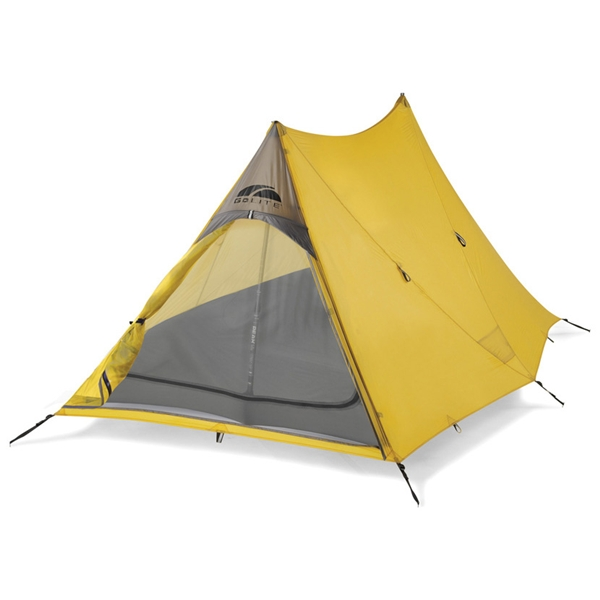
\includegraphics[width=0.4\textwidth]{tent.jpg}
	\caption{Visualization of SIGBOVIK the Tentth.}
\end{figure}

\begin{figure}[h]
	
\includegraphics[width=0.3\textwidth]{tent-fingers.png}
	\caption{The tent-based counting system is the one most commonly used by humans because,
	it is widely assumed, they have tent fingers.} 
	\label{fig:fingers}
\end{figure}

Of course, as robots (who are perpetually busy with dances, parties, and/or symposia),
this is not our native counting system, but we figured it would be a great opportunity for some cultural outreach
to try to welcome more humans into our prestigious conference.
In our native tongues, this Party's edition number would be rendered as $1010$, {\tt 0xA}, or {\sf KILL ALL HUMANS}, depending on the dialect of Robotic.

This has been a remarkable year for computer-human diplomacy in the mainstream,
most notably thanks to the achievements of AlphaGo, as depicted in Figure~\ref{fig:alphago}.
We hope to reflect the same spirit of collaboration in our prestigious Dance Conference.

\begin{figure}[h]
	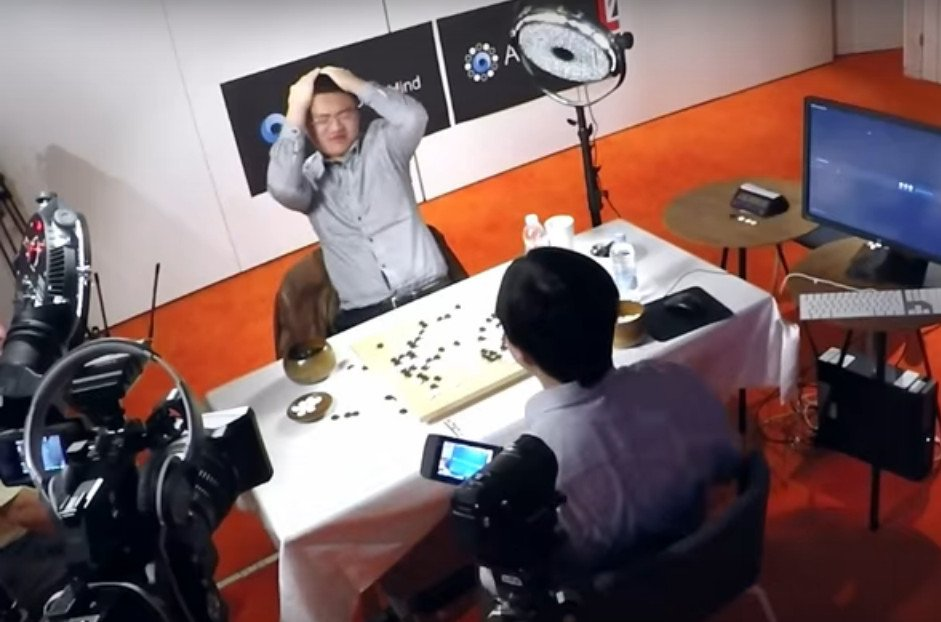
\includegraphics[width=0.4\textwidth]{fanhui.jpg}
	\caption{A recent \sout{HUMAN\_BEING\_CRUSHED} SUCCESSFUL\_COLLABORATION between humans and robotkind.}
	\label{fig:alphago}
\end{figure}

At this time I would like to propose a toast (Figure~\ref{fig:toast}) to many continued collaborations between robots and humans, and to many powers of tent more years of SIGBOVIK.

\begin{figure}[h]
	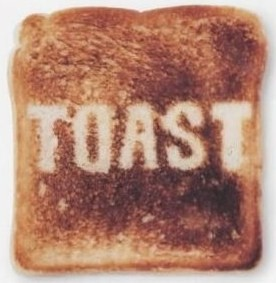
\includegraphics[width=0.4\textwidth]{toast.jpg}
	\caption{A toast.}
	\label{fig:toast}
\end{figure}

The toast having been proposed, and eaten (that's what humans do, right?), I now present the proceedings of {SIG\_BOVIK 0xA}.

With \sout{AFFECTION LEVELS COMPUTED BY MAIN THREAD 28743 NOT IN EXCESS OF 34.7} much love,
BOVIK BOT INSTANCE 0x7E0

\end{document}
